\documentclass{beamer} % "Beamer" is a word used in Germany to mean video projector [  

\usetheme{Berkeley} % Search online for beamer themes to find your favorite or use the Berkeley theme as in this file [ 



\usepackage{color} % It may be necessary to set PCTeX or whatever program you are using to output a  [ pdf instead of a  [ dvi file in order to see color on your screen [ 
\usepackage{graphicx} % This package is needed if you wish to include external image files [ 
\usepackage{hyperref}

\usepackage{amsmath}
\usepackage{amssymb}
\usepackage{amsthm}

\usepackage{amsmath}

\theoremstyle{definition} % See Lesson Three of the LaTeX Manual for more on this kind of "proclamation [ "
\newtheorem*{dfn}{A Reasonable Definition}               

\title{Image Steganography Analysis and Detection}
\author{Subalakshmi Shanthosi S} 
\institute{SSN College of Engineering}
\date{}
% Remove the % from the previous line and change the date if you want a particular date to be displayed; otherwise, today's date is displayed by default [ 

\AtBeginSection[]  % The commands within the following {} will be executed at the start of each section [ 
{
\begin{frame} % Within each "frame" there will be one or more "slides [ "  
\frametitle{Presentation Outline} % This is the title of the outline [ 
\tableofcontents[currentsection]  % This will display the table of contents and highlight the current section [ 
\end{frame}
} % Do not include the preceding set of commands if you prefer not to have a recurring outline displayed during your presentation [ 

\setbeamertemplate{sidebar right}{}
\makeatother

\setbeamertemplate{footline}
{
	\leavevmode%
	\hbox{%
		\begin{beamercolorbox}[wd=.333333\paperwidth,ht=2.25ex,dp=1ex,center]{author in head/foot}%
			\usebeamerfont{author in head/foot}\insertsection
		\end{beamercolorbox}%
		\begin{beamercolorbox}[wd=.333333\paperwidth,ht=2.25ex,dp=1ex,center]{title in head/foot}%
			\usebeamerfont{title in head/foot}\insertsubsection
		\end{beamercolorbox}%
		\begin{beamercolorbox}[wd=.333333\paperwidth,ht=2.25ex,dp=1ex,right]{date in head/foot}%
			\usebeamerfont{date in head/foot}\date[short date]{12-03-1019}\hspace*{2em}
			\insertframenumber{} / \inserttotalframenumber\hspace*{2ex} 
	\end{beamercolorbox}}%
	\vskip0pt%
}
\makeatletter
\setbeamertemplate{navigation symbols}{}
\date[short date]{12-03-2019}

\begin{document}

\begin{frame} 
\titlepage
\end{frame}

\section{What is Image Steganography?} % Since this is the start of a new section, our recurring outline will appear here 

\begin{frame} 
\frametitle{Image Steganography}
 \begin{itemize}
 \item{Steganography is the process of hiding a secret message within a
 larger one in such a way that someone can not know the presence or contents
 of the hidden message }
\end{itemize}
\begin{itemize}
 \item{Aim - To develop a detection system which is capable of detecting the alteration in image both its format and signature thereby predicting the actual type of forged file 
 }
\end{itemize}

\end{frame}

\begin{frame}
\frametitle{Challenges in Forged File Discovery}
 \begin{itemize}
	\item{Images without watermarking as digital signatures can be easily manipulated.}
\end{itemize}
\begin{itemize}
	\item{With the advent of new photo editing software - hiding critical informations are easy and unpercievable }
\end{itemize}
\begin{itemize}
	\item {Task to detect mix of scaled or compressed images as one is difficult}
\end{itemize}
\begin{itemize}
	\item{Incorporating machine learning techniques for feature analysis and decision making  to classify the image to be forged or not  
	}
   \item{Tamper detection to check for change in the file format extension}
\end{itemize}
\end{frame}

\section{Review Papers}
\begin{frame}
\frametitle{Image Steganography Review paper [1].}
\begin{itemize}
	\item{ A detailed literature review on a
		variety of different methods, algorithms, and schemes in image steganography is conducted in order to analyse and
		investigate them.
	}
   \item{Methods used:}
   \begin{itemize}
   	\item{Modified LSB(Least Significant Bit) Technique. }
   	\item{Modified LSB Technique with AES authentication mechanism.  }
   	\item{Steganography approach based on LSB in digital image.  }
   	\item{IMStego-Java based Tool with reduced PSNR in conventional LSB approach. }
   \end{itemize}
   \item{ Different Spatial and Transform techniques are realised.  }
   \item{Literature review demonstrating the popular steganographic techniques.}
\end{itemize}
\end{frame}

\begin{frame}
\frametitle{Digital Image Steganography Using Modified LSB and AES Cryptography[2].}
\begin{itemize}
	\item{ This method ensures enhanced security of digital images.  }
	\item {Steps involved:}
	\begin{itemize}
	\item{The secret message is transformed to cipher text by AES cryptography.}
	\item{ The cipher text is hidden inside the image using the modified LSB method.}
	\end{itemize}
	\item{Methods:Replacing LSB of cover image with the bits of the concealed message and manipulating the LSB plane of the cover image.}
	\item{Limitation :}
	\begin{itemize}
		\item {Less secure:Easy to decrypt secret message.}
		\item {Less performance.}
	\end{itemize}
	\item{Modified LSB shows improved performance based on PSNR,SSIM metrics.} 
	\item{Future work:Performance Improvement based on storage or computatational time.}
\end{itemize}
\end{frame}

\begin{frame}
 \frametitle{Image Steganography with Modified LSB and AES Encryption standards}
	\begin{figure}
		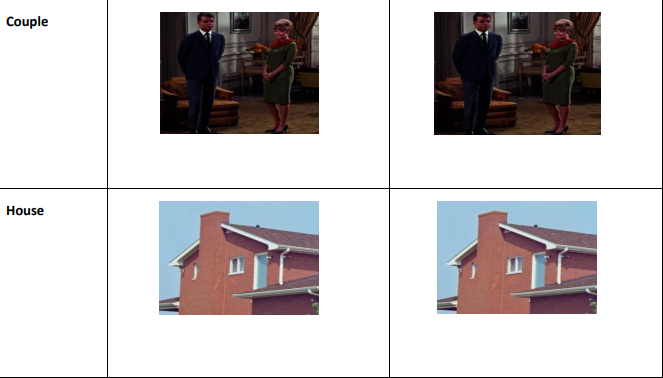
\includegraphics[scale=0.45]{modifiedLSB.png}
		\caption{Image Steganography with Modified LSB and AES Encryption standards}
	\end{figure}
\end{frame}

\begin{frame}
\frametitle{Boundary-based Image Forgery Detection by Fast Shallow CNN[3].  }
\begin{itemize}
	\item{ Network (SCNN) capable of distinguishing the boundaries of
		forged regions from original edges in low resolution images 
		SCNN is designed to utilize the information of chroma and
		saturation.}
	\item{Methods:Based on SCNN:}
	\begin{itemize}
		\item Sliding Windows Detection (SWD).
		\item Fast SCNN.
	\end{itemize}
	\item {Methodology:}
	\begin{itemize}
		\item{SWD: We start by picking a certain window of an image.}
		\item Window is feed into SCNN and compute a confidence score to predict whether it is tampered. 
		\item Confidence score and probablity map is maintained.   
		\item Then the window slides over and outputs another confidence score. 
		\item After sliding the window through the entire image, a complete probability map is constructed.
    \end{itemize}
\end{itemize}
\end{frame}

\begin{frame}
 \frametitle{Boundary-based Image Forgery Detection by Fast Shallow CNN[3] }
 \begin{itemize}
       \item{Fast SCNN :}
       \begin{itemize}
       	\item Takes entire image as the input  
       	\item Produces feature maps by processing the entire image
			with Conv layers.
		\item Extract feature vectors with dimension from feature maps and feed them into fully-connected layers. 
		\item The parameters of Fast SCNN are all trained by SCNN on
			the patch dataset.
		\end{itemize}
	\end{itemize}
\begin{itemize}
	\item{Limitation :}
	\begin{itemize}
		\item {Less secure:Easy to decrypt secret message. }
		\item {Less performance.  }
	\end{itemize}
	\item{Modified LSB shows improved performance based on PSNR,SSIM metrics.} 
	\item{Future work:Performance Improvement based on storage or computatational time.}
\end{itemize}
\end{frame}


\begin{frame}
\frametitle{Steganalysis of RGB Images Using Merged Statistical Features of Color Channels[4]  }
\begin{itemize}
	\item The steganalysis process is based on supervised machine learning, utilizing the Support Vector Machine (SVM) binary classifier’s implementation in MATLAB. 
	\item Proposed Model:
	\begin{itemize}
        \item{Based on merging features of single color channels into a multi-channel feature set, without consideration to the correlation between color channels.}
        \item{Accuracy of model is evaluated with uncompressed RGB clean image and stego image.}
     \item Feature Selection - Statistical Textural Features:
     \begin{itemize}
     	\item Single Channel - Statistical and Traditional Feature Set. 
     	\item Multi Channel -  Consists of GLCM features. Contrast,Correlation,Energy and Homogeneity, as well as other textural features such as Entropy in the study of textural features of images, and have been used in many steganalysis research works.
     \end{itemize}
	\end{itemize}
\end{itemize}
\end{frame}

\begin{frame}
\frametitle{Single Channel Features in Statistical Textural Features.  }
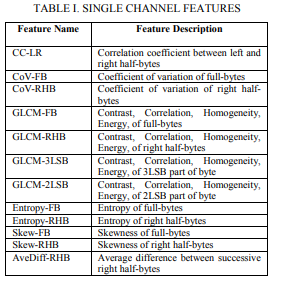
\includegraphics[scale=1.0]{singleChannelFeatures.png}
\end{frame}

\begin{frame}
\frametitle{Steganalysis of RGB Images Using Merged Statistical Features of Color Channels[4].  }
\begin{itemize}
	\item Dataset :  The selected cover image type is uncompressed RGB-BMP, in three channels, without the alpha channel.
	\item Two independent datasets are used, for double validation:
	\begin{itemize}
		\item The first validation dataset consists of 1500 clean images in TIFF format with alpha channel, that were downloaded from the Natural Resources Conservation (NRC) image dataset.
	    \item  The CALTECH’s birds images dataset [14], which is in a compressed color JPEG format .A set of 1500 CALTECH images were converted to BMP format and resized to 512 X 512 pixels.
	\end{itemize}
\end{itemize}
\end{frame}
\begin{frame}
\frametitle{Steganalysis of RGB Images Using Merged Statistical Features of Color Channels[4].}
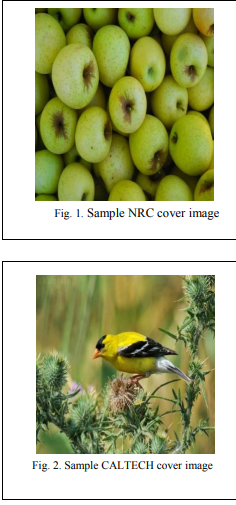
\includegraphics[scale=0.35]{nrcndcaltech.png}
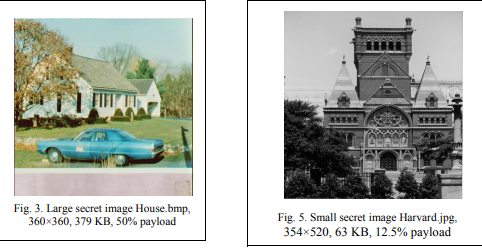
\includegraphics[scale=0.35]{stegImage.png}
\end{frame}

\begin{frame}
\frametitle{Steganalysis of RGB Images Using Merged Statistical Features of Color Channels[4].}
\begin{itemize}
\item Experimental Work:
 \begin{itemize}
 	 	\item Embedding : Secret messages are embedded using Spatial Steganography.
 	\begin{itemize}
 	\item Each Channel in each pixel were Embedded with 2 bits or 4 bits by replacing the least significant bits .For single channel embedding, only the NRC cover images were used, in which the Blue color channel of each pixel was embedded using 2-bpc.
 	\item  The processes of embedding have produced five stego datasets: NRC-LSB2, NRC-LSB4, CALTECH-LSB2, CALTECHLSB4, and NRC-2LSB-Blue.  
 \end{itemize}
      \item Features Extraction: Using build in functions of MATLAB. 
      \item Classification using SVM Classifier.
      \item Evaluation metrics :True Negative(TN),True Positive(TP), False Negative(FN) , False Positive(FP) and Detection Accuracy(DA).  
\end{itemize}
\end{itemize}
\end{frame}

\begin{frame}
\frametitle{Steganalysis of RGB Images Using Merged Statistical Features of Color Channels[4]. }
\begin{itemize}
\item Limitation: 
 \begin{itemize}
 	\item Does not apply to compressed images with lossey compression.
 	\item Performance and Storage consideration for Multi channel.
 	\item Capacity of hiding data is low.
 \end{itemize}
 \item Future Work : The proposed steganalysis model can be evaluated. using 
 \begin{itemize}
 	\item Lower embedding rates. 
 	\item Different media types : audio and video.  
 	\item Flexibility to work with transform domain.  
 \end{itemize}
 \end{itemize}
\end{frame}

\begin{frame}
\frametitle{Large-Scale JPEG Image Steganalysis Using Hybrid Deep-Learning Framework[5].}
\begin{itemize}
	\item Deep Learning in Image Steganalysis is still in its initial stage-A generic hybrid deep-learning framework for JPEG steganalysis incorporating the domain knowledge behind rich steganalytic models.
	\item Stages in JPEG Steganalysis:
	\begin{itemize}
		\item The first stage is hand-crafted, corresponding to the convolution phase followed by for rich model : 
		\begin{itemize}
            \item 	Quantization phase.  
            \item   Truncation phase.
		\end{itemize}
	    \item The second stage is a compound deep-neural network containing multiple deep subnets, in which the model parameters are learned in the training procedure. 
	\end{itemize}
\end{itemize}
\end{frame}
\begin{frame}
\frametitle{Large-Scale JPEG Image Steganalysis Using Hybrid Deep-Learning Framework[5]. }
\begin{itemize}
		\item Proposed Model:
	\begin{itemize}
		\item{Preliminaries: }
		\begin{itemize}
			\item 	The principal part of CNN is a cascade of alternating convolutional layers, regulation layers (eg. BN layers) and pooling layers.  
		\end{itemize}
\end{itemize}
\item Working : 
\begin{itemize}
	\item Each neuron unit receives inputs from a previous layer, performs a dot product with weights and optionally follows it with a nonlinear point-wise activation function .
	\item CNNs can be trained using backpropagation. 
\end{itemize}
\item Quantisation and Truncation in Steganalysis:
\begin{itemize}
	\item Convolution with series of kernal to derive varied noise residuals.
	\item Quantisation. 
	\item Truncation.
	\item Aggregation.  
\end{itemize}
\end{itemize}
\end{frame}

\begin{frame}
\frametitle{Large-Scale JPEG Image Steganalysis Using Hybrid Deep-Learning Framework[5]  }
\begin{itemize}
\item Hybrid Deep Learning Approach :
\begin{itemize}
	\item Takes Decompressed JPEG images and performes Convolution and Quantisation,Truncation.
	\item The second stage is a compound deep CNN network in which the model parameters are learned in the training procedure. 
\end{itemize}
\item Future Work : 
\begin{itemize}
	\item Incorporation of Adversarial Machine Learning into current hybrid framework. 
	\item Exploration of the application of hybrid framework in
	the field of multimedia forensics. 
\end{itemize}
\end{itemize}
\end{frame}

\begin{frame}
\frametitle{Large-Scale JPEG Image Steganalysis Using Hybrid Deep-Learning Framework[5].}

\begin{figure}
	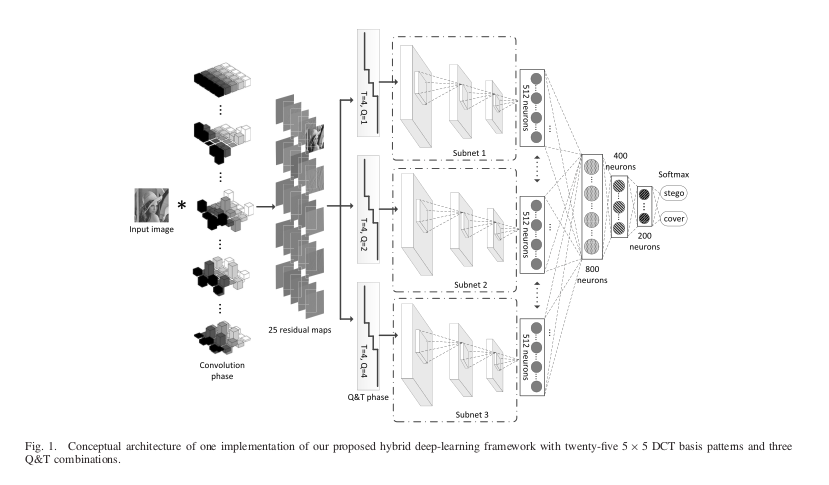
\includegraphics[scale=0.3]{jpegStegAnalysis.png}
	\caption{Hybrid Deep Learning Framework}
\end{figure}
\end{frame}


\section{Reference Papers}

\begin{itemize}
	\item{\textbf{Image Steganography Review paper [1]}, International Journal of Advanced Research in Computer and Communication Engineering(IJARCCE) , Mohammed A  Saleh ,\href{https://ijarcce.com/wp-content/uploads/2018/10/IJARCCE.2018.7910.pdf} {DOI}. }
\end{itemize}

\begin{itemize}
	\item{\textbf{Image Steganography Based on Modified LSB Substitution Method and Data Mapping[2]} ,   International Journal of Computer Science and Network Security(IJCSNS) , Pranab Kumar Dhar, Abdul Kaium and Tetsuya Shimamura , \href{http://paper.ijcsns.org/07_book/201803/20180321.pdf}{DOI} [ }
	\end{itemize}
\begin{itemize}
	\item{\textbf{Boundary-based Image Forgery Detection by Fast Shallow CNN[3]} , 2018 24th International Conference on Pattern Recognition (ICPR) , Zhongping Zhang , Yixuan Zhang , Zheng Zhou , Jiebo Luo , \href{https://doi.org/10.1109/ICPR.2018.8545074} {DOI} [  }

\end{itemize}

\begin{itemize}
	\item {\textbf{Steganalysis of RGB Images Using Merged Statistical Features of Color Channels[4]} , 2018 11th International Conference on Developments in eSystems Engineering (DeSE) , Zaid I.  Rasool , Mudhafar M.  Al-Jarrah ,Saad Amin , \href{https://doi.org/10.1109/DeSE.2018.00048}{DOI}. }
\end{itemize}
\begin{itemize}
	\item {\textbf{Large-Scale JPEG Image Steganalysis Using
			Hybrid Deep-Learning Framework[5]} ,  IEEE Transactions on Information Forensics and Security , Jishen Zeng  , Shunquan Tan  , Bin Li , Jiwu Huang , \href{https://doi.org/10.1109/TIFS.2017.2779446}{DOI. } }
\end{itemize}
\end{document}